\chapter{Introduction}
The intersection of physics and deep learning has never been more pronounced than it is today. With advancements in hardware and computational capabilities, we are now positioned to predict physical phenomena with unprecedented precision using deep learning techniques, particularly through physics-informed neural networks.\\
Physics-Informed Neural Networks (PINN) are neural networks  that encode model equations, like Partial Differential Equations (PDE), as a component of the neural network itself\cite{Cuomo2022}. For example let us take Laplace equation which is defined as
\begin{eqnarray}
	\Delta u(\mathbf{x}) &= 0, &\texttt{   }\mathbf{x}\in \Omega,\mathbf{x}\in R^2\\
	u &= S &\texttt{   }\mathbf{x}\in \partial\Omega \text{     Dirichlet boundary condition},\\
	\frac{\partial u}{\partial \mathbf{n}} &= f(\mathbf{x}) &\texttt{   }\mathbf{x}\in \partial\Omega \text{     Neumann boundary condition}.
\end{eqnarray}
The Operator $\Delta$ is called as Laplace Operator and it defines $\Delta = \sum_i \frac{\partial^2}{\partial^2 x_i}.$\\
The $\Omega$ is domain and $\partial \Omega$ is boundary of the domain. 
To build a PINN model we will use an neural network which will learn the solution $u$ and from that output we will calculate all needed derivatives, residuals and other parts for the optimization.

\begin{figure}[h!]
	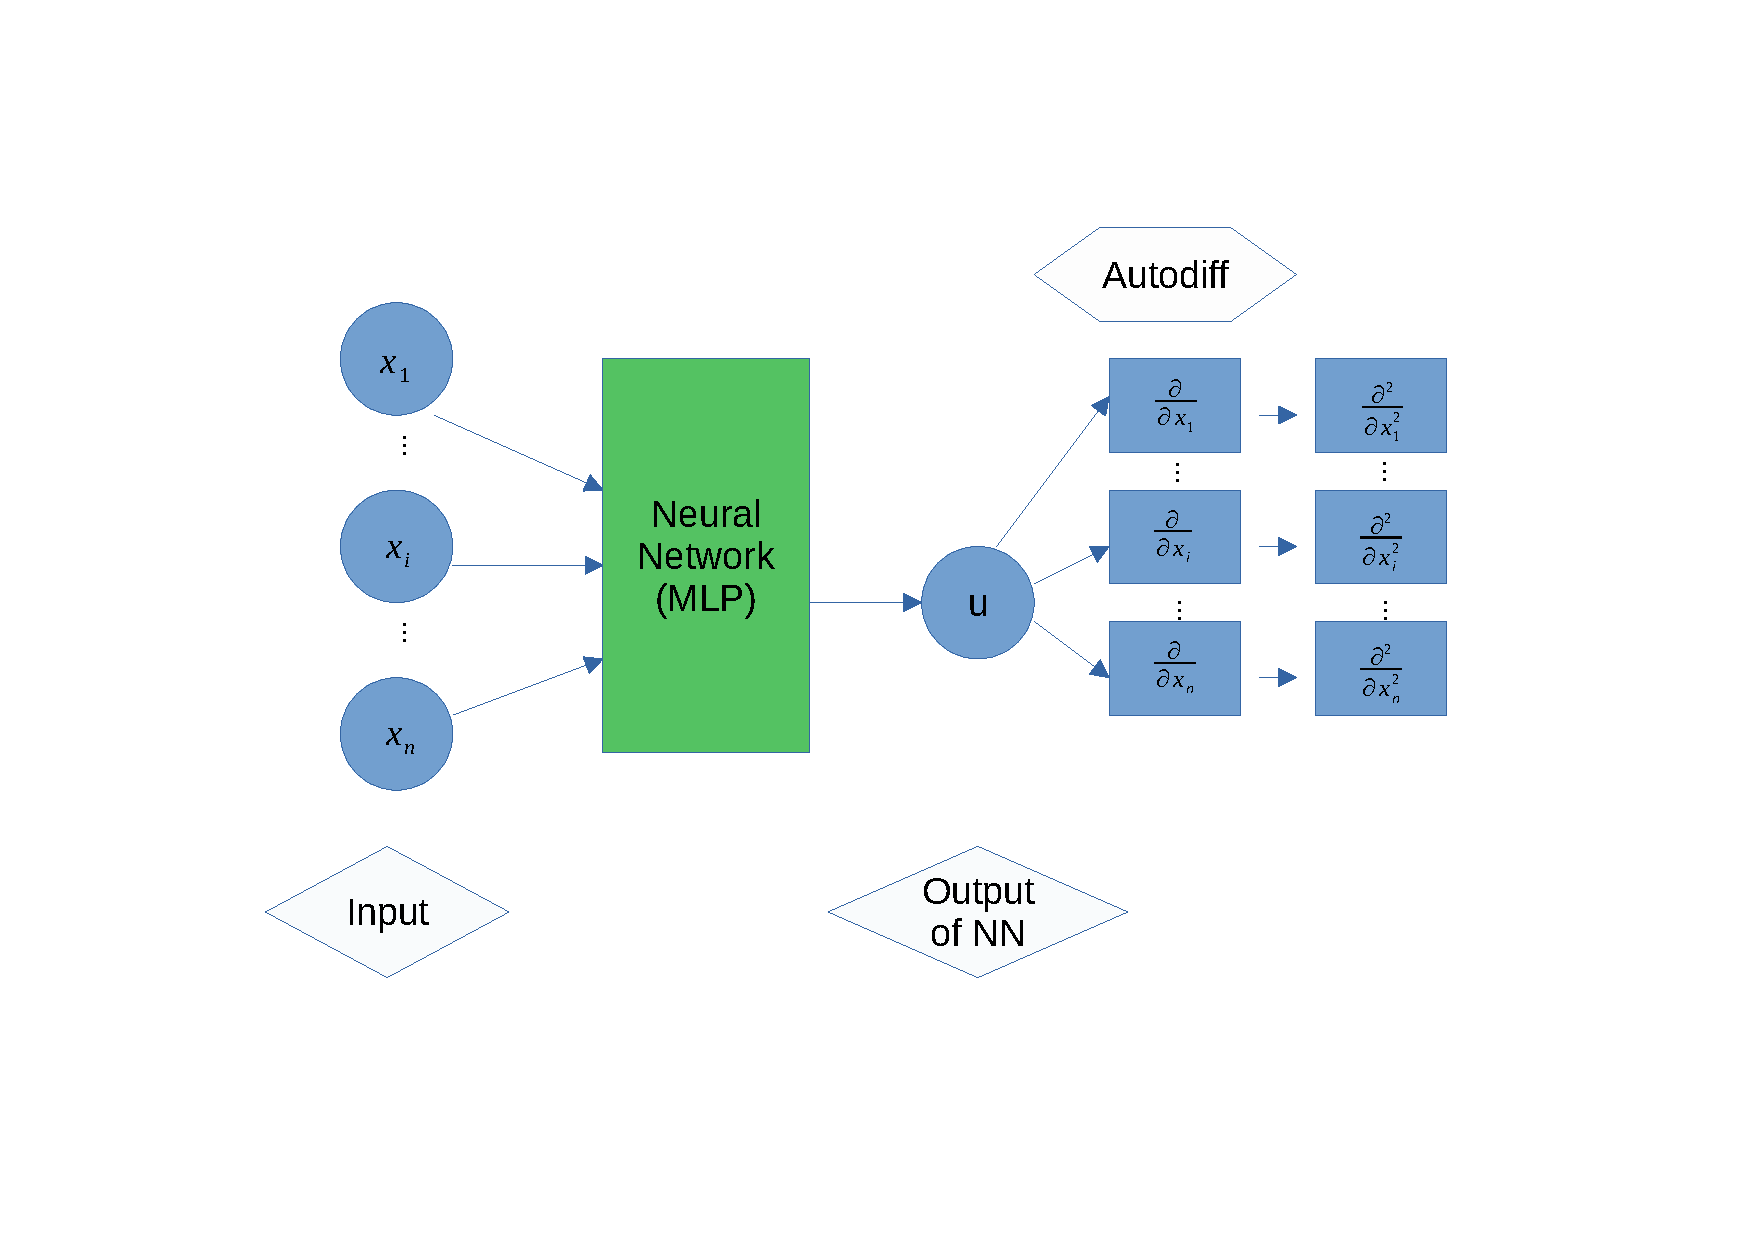
\includegraphics[width=15cm]{chapters/chapter1/pinn}
	\caption{PINN model for Laplace Equation}
	\label{a}
\end{figure}
In figure \ref{a} we can observe the architecture of such physics informed model. 
The Loss functions that we need to use to properly train our network are
\begin{eqnarray}
	\text{Loss}_s(\Theta) &=& \frac{1}{N}\sum^N_i\left(u_{\Theta}(\mathbf{x}_i)- u_i\right)^2,\\
	\text{Loss}_r(\Theta) &=& \frac{1}{R}\sum^R_i\left(\frac{\partial u_{\Theta}(\mathbf{x}_i)}{\partial x_i} - f(\mathbf{x}_i)\right)^2,\\
	\text{Loss}_l(\Theta) &=& \Delta u_{\Theta},\\
	\text{Loss}(\Theta) &=& \omega_s \text{Loss}_s +\omega_r \text{Loss}_r +\omega_l \text{Loss}_l .
\end{eqnarray}
The laplace equation is often used to calculate or describe physical phenomena which are bounded to domain, like electrical fields. The domain $\Omega$ needs to be discretisized.
With given discretization we divide $R$ as number of $\mathbf{x}_i$ which are on the boundary of the domain and $N$ the Number of all $\mathbf{x}_i$ in $\Omega$.
The $\omega_s$,$\omega_r$,$\omega_l$, in this case are coefficients $0\leq \omega \leq 1$ and they are there to improve optimization capabilities which is defined as
\begin{equation}
	\Theta^* = \arg\min\text{Loss}(\Theta).
\end{equation}
The $\Theta$ are learnable parameters which can be updated with $\Theta^*$ trough optimization algorithm.\\
Such model wouldn't be possible without automatic differentiation\cite{autodiff} which is offered from machine learning library $\texttt{pytorch}$\cite{pytorch}. In this example we need a large amount of data, and the optimization of the model could be very slow,especially if we don't have a computation capable hardware for it. Obtaining the data can be done trough precise measurement or using some numerical solvers like FEM\cite{fem} or Isogeometric Analysis\cite{iga}. Keep in mind that there are Poission Equation, Wave Equation which are time-dependent $t$.\\
Those PDEs are mostly appllied in electrotechnical(Electro-magnetical fields) and  civil Engineering(static in construction).
In this thesis we won't work on the PDEs but in similar vein, we will try to train a model to predict the Dynamics of some physical phenomena and non-/holonomic hamiltonian systems.\\
The Dynamics for Robots called Joint Space Dynamics are defined as second order ordinary differential equation\cite{jointspace} .
\begin{equation}
	\mathbf{M}\ddot{\mathbf{x}}(t) + \mathbf{D}(\dot{\mathbf{x}}(t)) + \mathbf{C}(\mathbf{x}(t))=\tau,
\end{equation} but there are other forms, as Langrange Equations of Motion if our system is holonomic\cite{holo}. It is based on Lagrange Function which is based on Kinetic $T$ and Potential $U$ Energy
\begin{eqnarray}
	\mathcal{L} &=& T - V,\\
	\frac{d}{dt}\frac{\partial \mathcal{L}}{\partial \dot{q}_i} - \frac{\partial \mathcal{L}}{\partial q_i}&=&0.
\end{eqnarray}   
The Lagrange Equations are used in Deep Langrangian Networks\cite{delan}. In simillar manner, there are Hamiltonian Equations of Motion.
They work for holonomic and non-holonomic hamiltonian systems and they are capable to build first order ordinary equation
\begin{equation}
	\dot{x} = f(x,t)
\end{equation} \\
or in Hamiltonian Form where $\mathcal{H} = T + V$
\begin{equation}
	\dot{\mathbf{z}} = \mathbf{J}\frac{\partial\mathcal{H}}{\partial \mathbf{z}}(\mathbf{z})
\end{equation} where $\mathbf{z}=[\mathbf{q},\mathbf{p}]^T$ and $\mathbf{J} = \begin{bmatrix}
0 & \mathbf{I}_n\\
-\mathbf{I}_n & 0
\end{bmatrix} $\\
\begin{figure}[h!]
	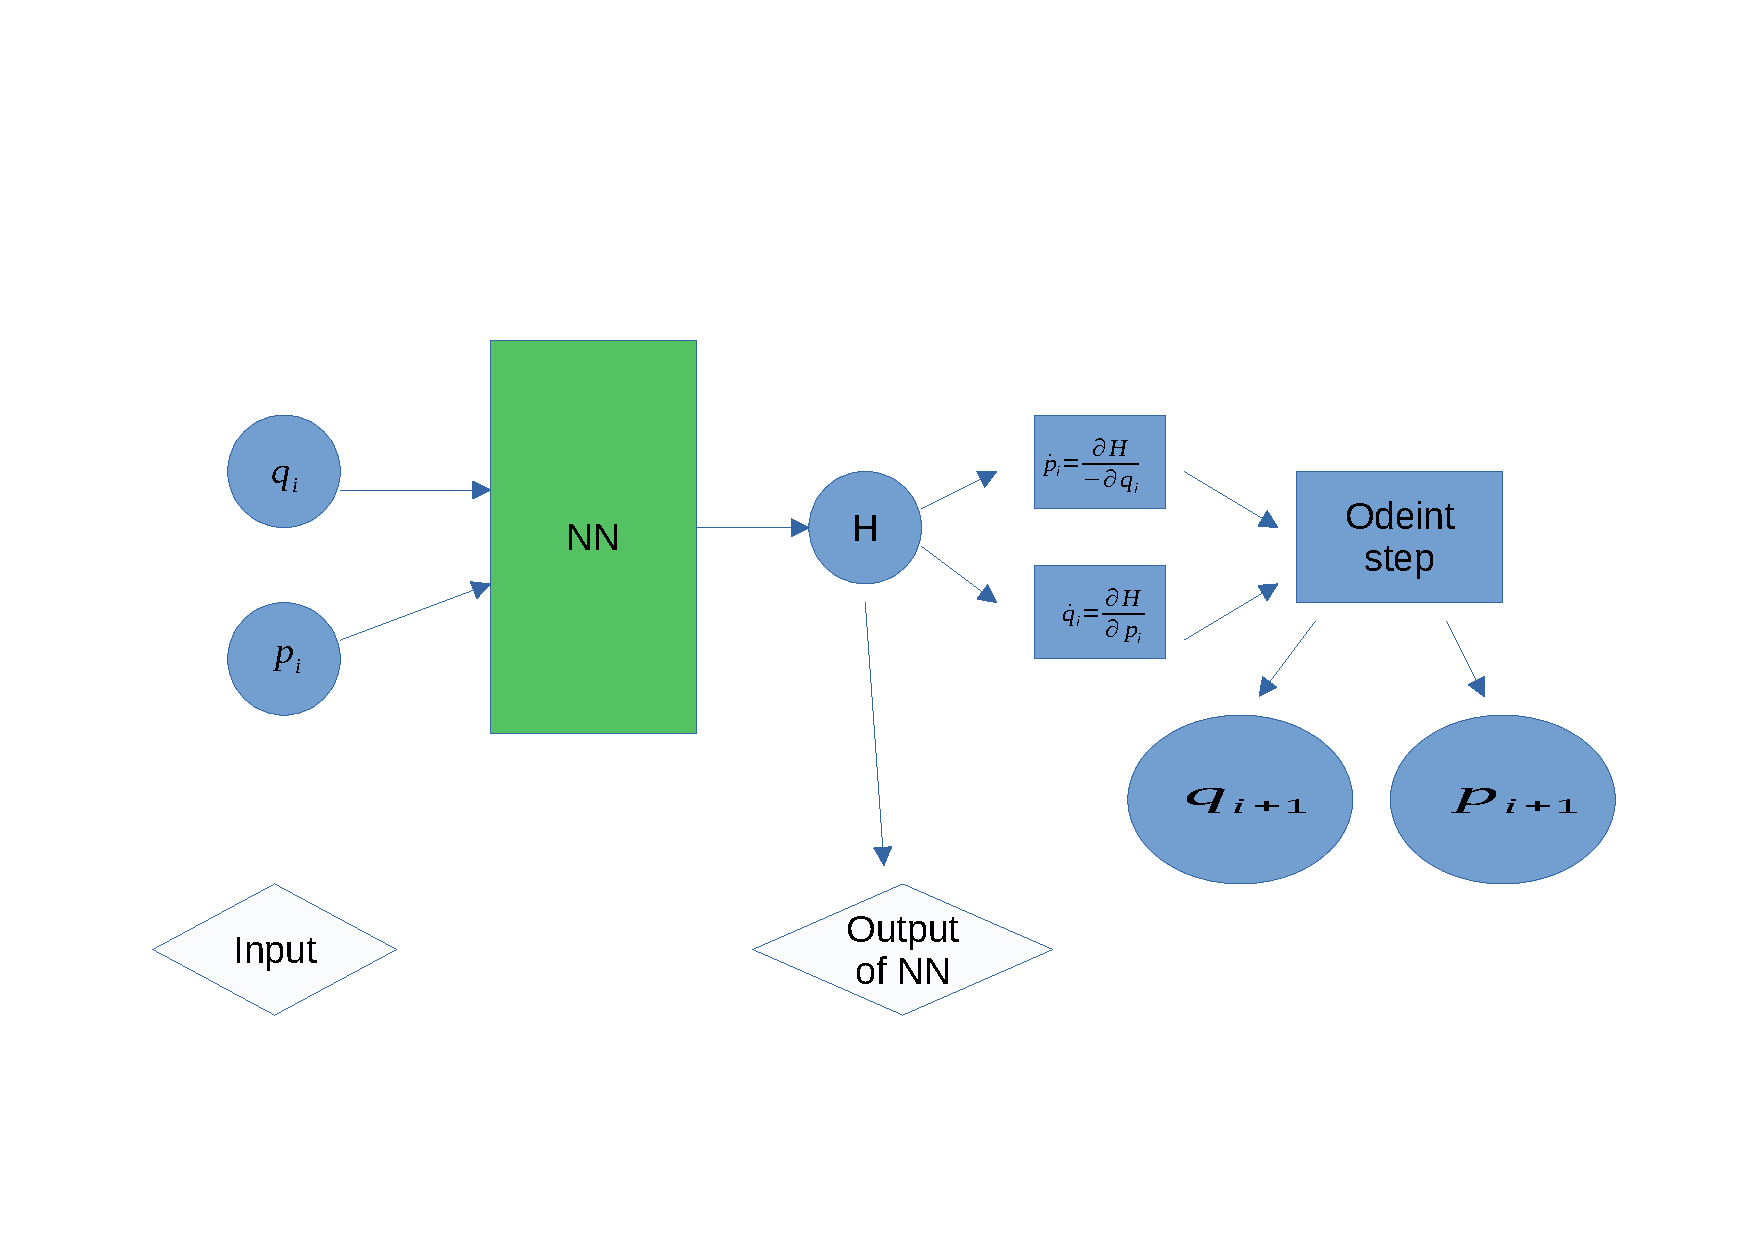
\includegraphics[width=15cm]{chapters/chapter1/hnn}
	\caption{HNN model with integration solver step}
	\label{fig:hnn}
\end{figure}
One of such model is introduced in the \cite{hnn} and it is called Hamiltonian Neural Network. it architecture you can observe in figure \ref{fig:hnn}.
We will make it more interesting introducing the Graph Neural Network instead Conventional Multy layer Perceptron and try to use it as a base of our architecture. We hypothesize that implementing a Graph Neural Network could improve the architecture's performance. 
In this thesis, we will also discuss Hamiltonian equations and how to derive them. During our research, we encountered the issue that there are no high-quality datasets available for training physics-based neural networks. Given this, we will explain how to create five datasets based on Hamiltonian Equations of Motion.\\
Next we will revisit state of the art neural architectures and test NeuralODE as new Nerual Paradigm, and how thy learn dynamics from given data.\\
In the experiments we tested the capabilities of Graph Neural Networks based PINN Models, how do they adapt to diverse training data and their possibility to reduce or increase a degree of freedom in the training. For example how similar is the movement between 3 and 4 bodied pendulum on the same trained set of neural parameters. We hope that we will give valuable insight in those topics.    








%% related works, philosophy, motivations, my contributions
